%!TEX root = Main.tex

\section{Simulation} \label{sec:simulation}


\begin{figure}[H]
\includegraphics[width=\textwidth]{../simulation/plots/center_pdfarray_confband}
\caption{Connecting patterns.}
\end{figure}



\begin{figure}[H]
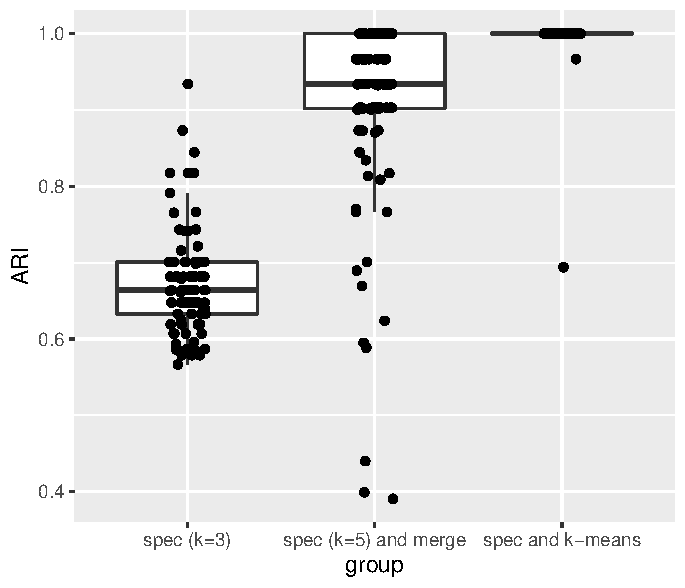
\includegraphics[width=.8\textwidth]{../simulation/plots/Boxplot_cmpr}
\caption{Clustering result.}
\end{figure}


\begin{figure}[H]
\begin{subfigure}{.49\textwidth}
\includegraphics[width=\textwidth]{../simulation/plots/overclus_a}
\caption{}
\end{subfigure}
\begin{subfigure}{.49\textwidth}
\includegraphics[width=\textwidth]{../simulation/plots/overclus_c}
\caption{}
\end{subfigure}
\begin{subfigure}{.49\textwidth}
\includegraphics[width=\textwidth]{../simulation/plots/overclus_b}
\caption{}
\end{subfigure}
\begin{subfigure}{.49\textwidth}
\includegraphics[width=\textwidth]{../simulation/plots/overclus_d}
\caption{}
\end{subfigure}
\caption{(a): 2 dimensional representation of aggregated point processes.
(b): Result of spectral clustering with three clusters.
(c): Result of spectral clustering with five clusters.
(d): Result of merging the five clusters into three. }
\end{figure}










% \subsection*{Over-clustering does not always help}
% Possible reasons:
% \begin{itemize}
% 	\item Makes some clusters too small, the estimate for connecting patterns get worse.
% 	\item Spectral clustering does not keep hierarchical structure, over-clustering may get worse clustering results.
% 	\item Individual connecting patterns are similar after eliminating  time lags between groups, so different (but similar) groups might be merged together. 
% \end{itemize}






% \subsection*{Remark}
% \begin{enumerate}
% \item Using pdf can avoid getting large distance between curves with similar shapes but different peak heights
% \item Smoothing can cause non-identifiability of uniform distribution and normal distribution.
% \item A bigger size of clusters can lead to a better smooth result.
% \item When combining subjects, consider the biological clock?
% \item Spectral clustering does not keep hierarchical structure.
% \end{enumerate}

% In the first case we analyze the network with two types of nodes.
% Figure \ref{fig: nodes locations} shows the locations of 50 nodes, among which 4 are from type I and the rest 46 are from type II.
% The first type of nodes (type I) are generated uniformly from $[0.3, 0.7]\times[0.8, 5.2]$.
% The second type of nodes (type II) are generated uniformly in $[0,1]\times[0,6]$. 
% \\

% \noindent
% The network is developed during time period $[0,50]$.
% Two nodes are connected if the distance between them is less than $1$.
% The connecting time between two type II nodes is generated from uniform distribution $U(0,40)$.
% For the pair of nodes with one from type I and the other from type II, the connecting time is distributed as $N(5+\tau,1)$, where $\tau$ is the time delay caused by the type I node and is generated randomly from $U(0,30)$.





% The second case is with three clusters.
% The locations of nodes are displayed in Figure \ref{fig: nodes locations, case 2}.
% The connecting radius for type I node is set as $2$, and that for other nodes is set as $1$. 
% For a pair of type III nodes, the connecting time is generated from uniform distribution $U(0,30)$.
% For the pair of nodes with one from type II and the other from type III, 
% the connecting time is distributed as $N(5+\tau,1)$, where $\tau$ is the time delay caused by the type II node and is generated randomly from $U(0,5)$.
% For the pair of nodes with one from type I and the other from type II, the connecting time is distributed as $U(\tau,\tau+6)$, where $\tau$ is the time delay caused by the type II node and is generated randomly from $U(40,42)$.




